%
% Copyright (c) 2017  Zubax Robotics OU  <info@zubax.com>
%
% Distributed under BY-NC-ND (attribution required, non-commercial use only, no derivatives).
%

\documentclass{zubaxdoc}
\graphicspath{{document_templates/documentation_template_latex/}}

\usepackage{ConfigParamIndex}
\usepackage{amsmath}
\usepackage{textcomp}

\title{Zubax Babel Datasheet}

\hbadness=10000

\begin{document}
\frontmatter
\begin{titlepage}

\section*{Overview}

Zubax Babel is an advanced USB-\allowbreak{}CAN and UART-\allowbreak{}CAN adapter
that can be used as a standalone device or as an embeddable module for
OEM\footnote{Original equipment manufacturer.}.

Babel uses the quasi-standard SLCAN (aka LAWICEL) protocol (with Zubax extensions)
for transferring CAN data over USB and UART.
There is a wide selection of software products that can communicate with SLCAN-compatible adapters.

\section*{Features}

\begin{itemize}
    \item Very low latency -- the cumulative latency between the host system
          and the CAN bus is under 1 millisecond.\footnote{Tested via USB on Linux 3.13
          using the low-latency SLCAN driver from the PyUAVCAN library.}

    \item Very high throughput -- the device handles more than 5000 frames per second in either direction
          continuously.\footnote{Tested via USB on Linux 3.13.
          When using the UART interface, the throughput is limited by the UART baud rate setting.}

    \item Large RX buffer (255 CAN frames plus 2KB of serial buffers) allows the device to handle short-term
          traffic bursts regardless of the throughput of the host-side interface.

    \item Proper prioritization of the outgoing CAN frames.
          The adapter properly schedules the outgoing frames, avoiding the inner priority inversion problem
          in the TX queue.

    \item Embedded 120~$\Omega{}$ CAN bus termination resistor that can be turned on and off by a command.

    \item Embedded CAN bus power supply output that can be turned on and off by a command.

    \item CAN bus supply voltage monitoring.

    \item SMD soldering pads for OEM applications.
\end{itemize}

\BeginRightColumn

\section*{Applications}

\begin{itemize}
    \item General-purpose USB-CAN or UART-CAN adapter.
    \item Diagnostic, monitoring, and development tool for \href{http://uavcan.org}{UAVCAN} networks.
          We recommend the UAVCAN GUI Tool for use with UAVCAN applications.
    \item Generic CAN/UAVCAN development board.
    \item Programmable CAN unit in OEM applications.
\end{itemize}

\centering{
    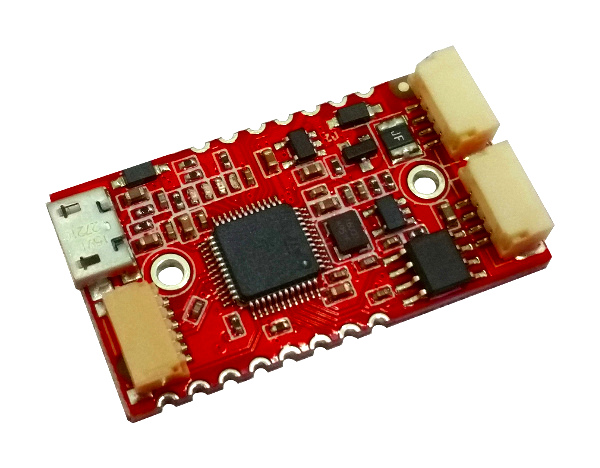
\includegraphics[width=0.45\textwidth]{top}
    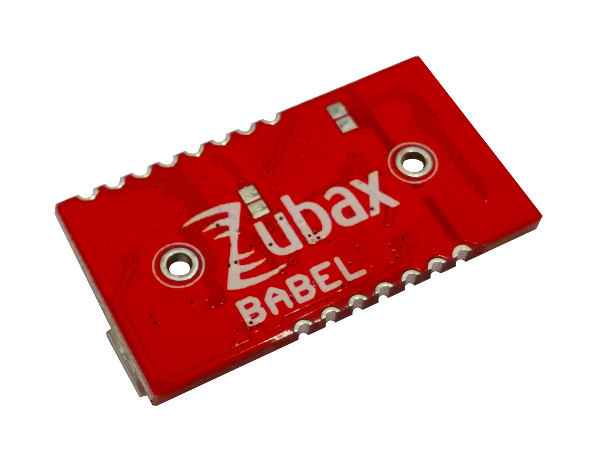
\includegraphics[width=0.45\textwidth]{bottom}
}

\end{titlepage}

\tableofcontents
\BeginRightColumn
\listoffigures
\listoftables

\mainmatter

\chapter{Overview}

Zubax Babel is an advanced USB-CAN and UART-CAN adapter
that can be used as a standalone device or as an embeddable module for
OEM.

\section{Accessories}

Zubax Babel can be used with the following accessories:
\begin{itemize}
    \item Plastic enclosure described in the section \ref{sec:enclosure}.
    \item UAVCAN cabling and related items.
    \item Standard USB cables.
    \item Cables compatible with the Dronecode Autopilot Connector Standard.
\end{itemize}

Please contact your supplier for the ordering information.

\subsection{Enclosure}\label{sec:enclosure}

Zubax Babel can be enclosed into a plastic enclosure pictured on the figure \ref{fig:enclosure}.
The enclosure provides a mechanical protection that makes the device more suitable for use as a
general-purpose desktop CAN adapter tool.

\begin{figure}[hb]
    \centering
    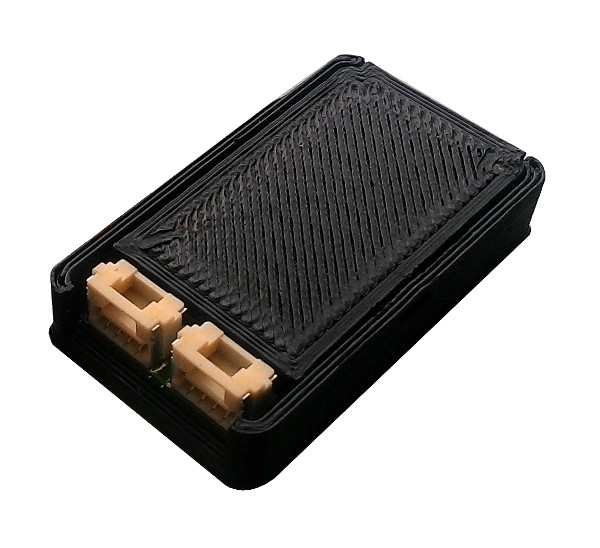
\includegraphics[width=0.45\textwidth]{housing}
    \caption{Plastic enclosure.\label{fig:enclosure}}
\end{figure}

Please contact your supplier for the ordering information;
alternatively, visit the website at \mbox{\url{https://github.com/Zubax/zubax_babel}} to download
3D-printable enclosure models suitable for in-house manufacturing.

\section{Quality assurance}

Every manufactured Babel undergoes an automated testing procedure that validates that
the device is functioning as designed.
The test log for every manufactured device is available on the web at
\url{https://device.zubax.com/device_info}.
This feature can be used to facilitate traceability of purchased devices and
provide additional safety assurances.

Every manufactured device has a strong digital signature stored in its non-volatile memory
which proves the origins of the product and eliminates the risk of sourcing unlicensed or
counterfeit hardware.
This signature is referred to as Certificate of Authenticity (CoA).
Please refer to the \href{https://kb.zubax.com}{Zubax Knowledge Base} to learn more about
the certificate of authenticity and how it can be used to trace the origins of your hardware.

\chapter{Characteristics}

\section{Absolute maximum ratings}

Stresses that exceed the limits specified in this section may cause permanent damage to the device.
Proper operation of the device within the limits specified in this section is not implied.

\begin{ZubaxSimpleTable}{Absolute maximum ratings}{|c X|c c|c|}
    Symbol            & Parameter                & Min  & Max & Unit \\
    $V_\text{supply}$ & Supply voltage           & -0.3 & 6   & V \\
    $T_\text{oper}$   & Operating temperature    & -40  & 85  & \degree{}C \\
	              & UART RX input voltage    & -0.3 & 6   & V\\
	              & CAN H/L input voltage    & -4   & 16  & V\\
\end{ZubaxSimpleTable}

\section{Environmental conditions}

\begin{ZubaxTableWrapper}{Environmental conditions}
    \begin{ZubaxWrappedTable}{|c X|l c|c|c|}
        Symbol            & Parameter                     &  Min & Max & Unit \\
        $T_\text{oper}$   & Operating temperature         & -40  & 85  & \degree{}C \\
        $T_\text{stor}$   & Storage temperature           & -40  & 85  & \degree{}C \\
        $\phi_\text{oper}$& Operating humidity\tnote{a}   & 0    & 100 & \%RH\\
    \end{ZubaxWrappedTable}
    \begin{tablenotes}
        \item[a] Condensation not permitted.
    \end{tablenotes}
\end{ZubaxTableWrapper}

\section{Power supply}\label{sec:power}

Babel requires a +5 V DC power supply input
which can be delivered via any of the available interface connectors.

The device has a reverse current protection on the USB power input
which prevents back-powering the USB host when it is turned off.

The CAN power output has a solid state switch that can be enabled and disabled
by setting the configuration parameter \CfgRef{can.power+on}.
The device can always be powered from the CAN bus regardless of the state of the power switch.

An additional +3.3 V DC output on the SMD pads can be used to power an external circuitry when the device
is used as a development board or in OEM applications.
The pinout specification for the SMD pads is provided in the section \ref{sec:smd_pads}.

The topology of the power supply circuits is documented on the figure \ref{fig:power_supply_scheme}.
Power input and output capabilities per interface are summarized in the table \ref{table:power_supply_summary}.

\begin{figure}[!hbt]
    \centerline{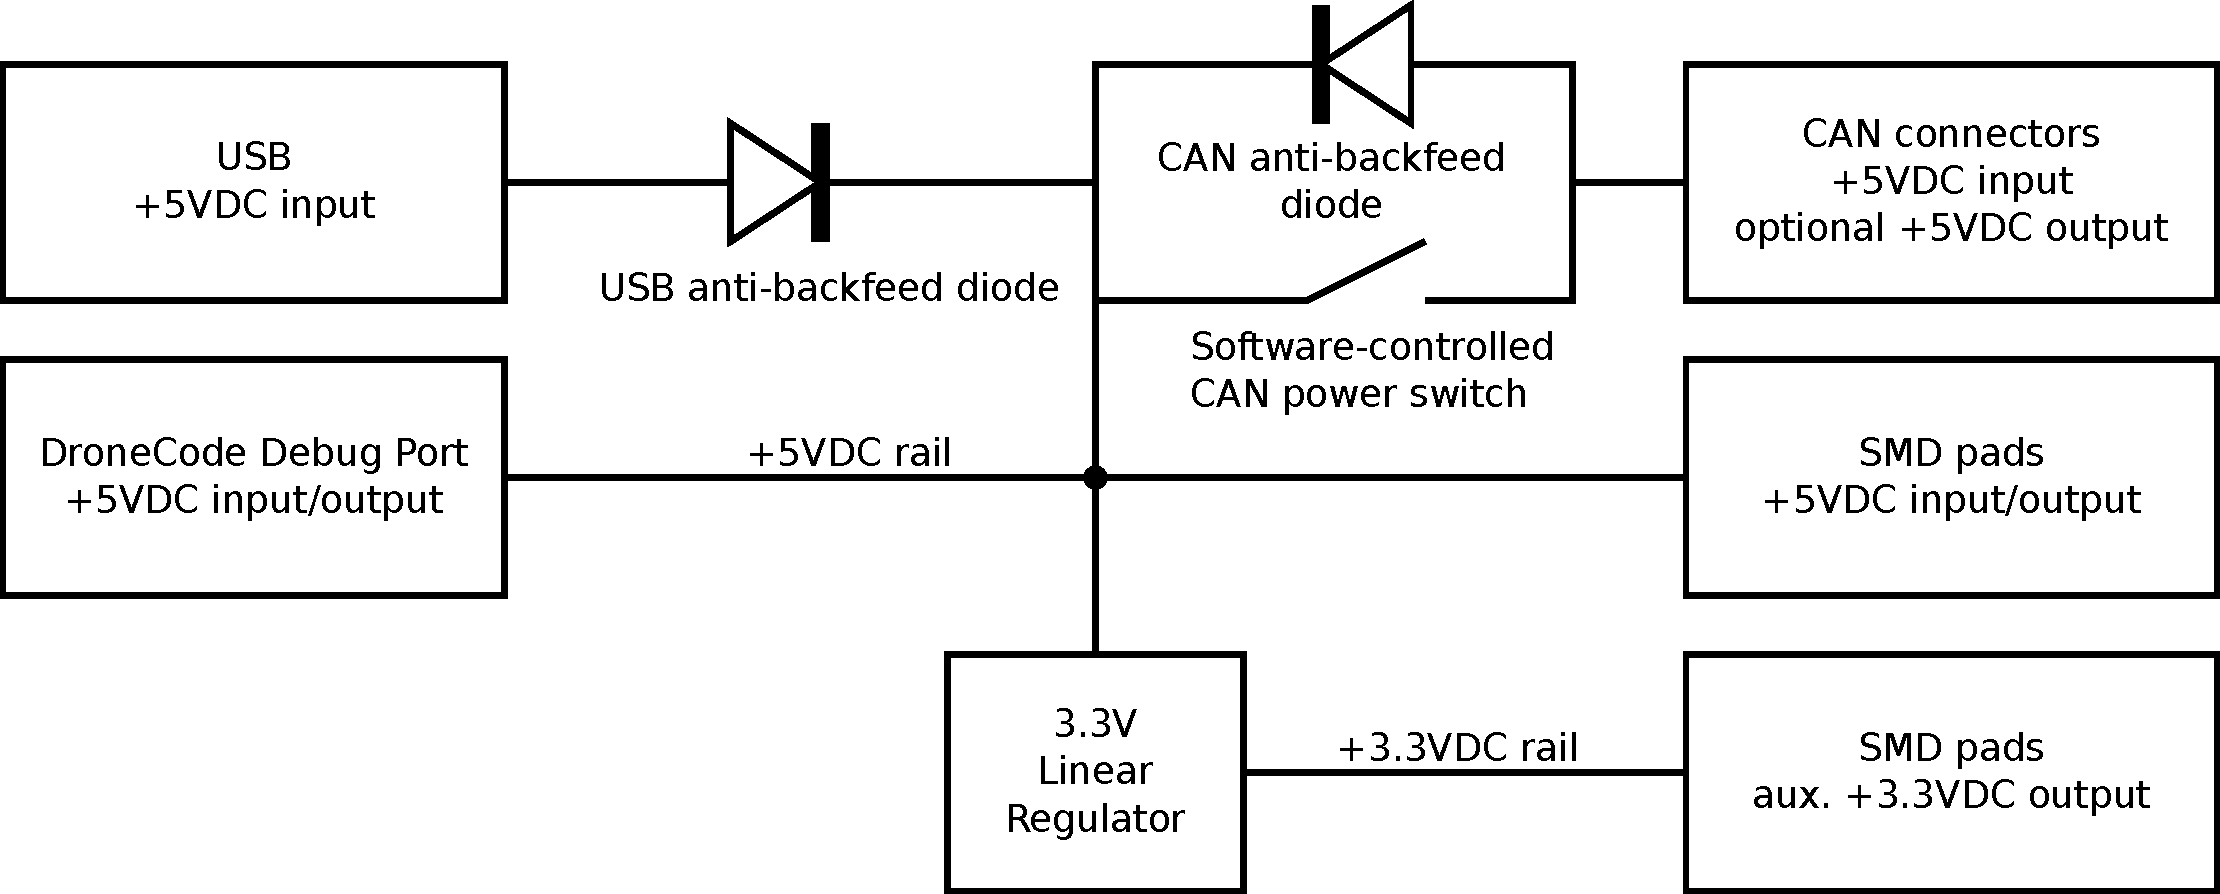
\includegraphics[width=1\textwidth]{power_supply}}
    \vspace{1em}
    \caption{Power supply architecture.\label{fig:power_supply_scheme}}
\end{figure}

\begin{ZubaxSimpleTable}{Power supply summary}{|l X X|}\label{table:power_supply_summary}
    Interface            & Direction              & Section \\
    CAN                  & Input, optional output & \ref{sec:can_bus} \\
    USB                  & Input                  & \ref{sec:usb} \\
    Dronecode debug port & Input, output          & \ref{sec:dronecode_debug_port} \\
    SMD pads             & Input, output          & \ref{sec:smd_pads} \\
\end{ZubaxSimpleTable}

\begin{ZubaxTableWrapper}{Power supply characteristics}
    \begin{ZubaxWrappedTable}{|c X| c c c | c|}\label{table:power}
        Symbol            & Parameter                 & Min & Typ & Max & Unit \\
        $V_\text{supply}$ & Supply voltage\tnote{a}   & 4.0 & 5.0 & 5.5 & V  \\
        $I_\text{supply}$ & Supply current\tnote{b}   & 30  & 50  & 80  & mA \\
                          & 3.3 V rail output voltage & 3.2 & 3.3 & 3.4 & V  \\
                          & 3.3 V rail external load  &     &     & 100 & mA \\
    \end{ZubaxWrappedTable}
    \begin{tablenotes}
        \item[a] Any power input.
        \item[b] SMD pads floating, Dronecode port disconnected.
    \end{tablenotes}
\end{ZubaxTableWrapper}

\section{Communication interfaces}

Zubax Babel features a variety of communication interfaces that facilitate easy integration into various
applications:
\begin{itemize}
    \item CAN 2.0A/B (ISO 11898).
    \item USB port (CDC ACM, virtual serial port).
    \item Dronecode debug port.
    \item SMD pads for OEM applications.
\end{itemize}

\subsection{CAN bus}\label{sec:can_bus}

Zubax Babel implements the ISO 11898 CAN 2.0 A/B bus physical layer standard, also known as high-speed CAN.
The CAN bus interface is equipped with two standard
UAVCAN Micro connectors (JST GH)\footnote{\url{https://kb.zubax.com/x/EoAh}}
electrically parallel to each other,
which facilitates easy integration of the device into the end application without the need to use T-connectors.

The default bit rate of the CAN bus can be set via the configuration parameter \CfgRef{can.bitrate},
in bits per second.

Babel always attempts to configure the CAN timings so as to achieve settings as close as possible to the
following:
\begin{itemize}
    \item Sampling point location: 87.5\%.
    \item Time quanta per bit: 8--10 for bit rate $\geq$ 1 Mbps, 16--17 otherwise.
    \item Resynchronization jump width: 1 time quantum.
\end{itemize}

The CAN interface recovers from the bus-off state automatically once the controller has
observed 128 occurrences of 11 consecutive recessive bits on the bus, as defined by the CAN specification.

The device has an embedded 120 $\Omega$ CAN termination resistor that can be enabled and disabled
by setting the configuration parameter \CfgRef{can.terminator+on}.
Changes to this configuration parameter take effect immediately.

The power switch, when turned on, delivers a +5 V DC supply to the CAN bus,
which can be used to power other CAN bus nodes from Zubax Babel
(section \ref{sec:power}).
The power switch is controlled by the configuration parameter \CfgRef{can.power+on}.
Changes to this configuration parameter take effect immediately.

The physical locations of the CAN connectors are documented in the section \ref{sec:mechanical}.

\subsubsection{Device interconnection}

The figure \ref{can_daisy_chain} shows a typical CAN bus topology.
Observe that if Babel is a last device on the bus, a separate termination resistor would not be necessary,
since Babel has an embedded termination resistor that can be enabled by setting the configuration
parameter \CfgRef{can.terminator+on}.

The CAN bus interface of Babel is not redundant.
If redundancy is desired, multiple Babels should be used in parallel, one per bus.

\begin{figure}[hbt]
    \centering
    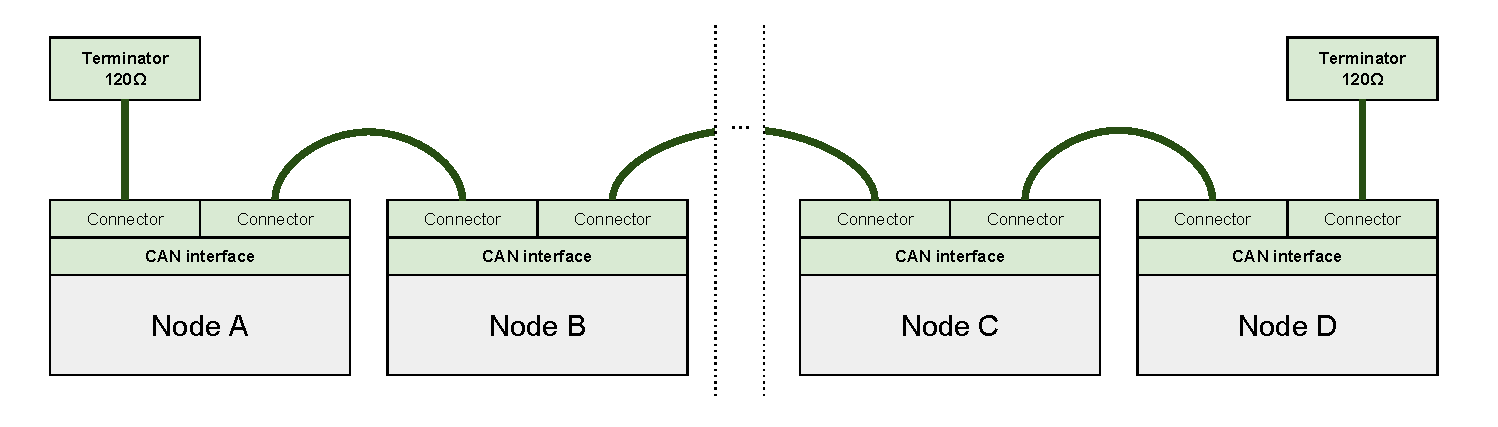
\includegraphics[width=1\textwidth]{can_daisy_chain}
    \caption{CAN bus interconnection diagram.
    \label{can_daisy_chain}}
\end{figure}

\subsubsection{Characteristics}

\begin{ZubaxTableWrapper}{UAVCAN Micro (JST GH) standard connector pinout}
    \begin{ZubaxWrappedTable}{|l X X[2]|}
        Pin no. & Type            & Function\\
        1       & Power           & +5 V power supply output and/or pass-trough\tnote{a}\\
        2       & Input/output    & CAN High\\
        3       & Input/output    & CAN Low\\
        4       & Ground          & Power \& signal ground\\
    \end{ZubaxWrappedTable}
	\begin{tablenotes}
	    \item[a] Power output be enabled/disabled by setting the configuration parameter \CfgRef{can.power+on}.
	\end{tablenotes}
\end{ZubaxTableWrapper}

\begin{ZubaxTableWrapper}{CAN bus interface characteristics}
	\begin{ZubaxWrappedTable}{|c X|c c c|c|}
		Symbol  & Parameter                                 & Min  & Typ  & Max  & Unit \\
		        & Bit rate                                  &      &      & 1000 & Kbps \\
		        & Positive-going input threshold voltage    &      & 750  & 900  & mV \\
		        & Negative-going input threshold voltage    & 500  & 600  &      & mV \\
		        & Differential output voltage, dominant     & 1.5  & 2.0  & 3.0  & V \\
		        & Differential output voltage, recessive    & -120 & 0    & 12   & mV \\
		        & Inter-connector current pass-through\tnote{a}& -1&      & 1    & A \\
		        & Connector resistance during device lifetime &    & 30   & 50   & $\text{m}\Omega$ \\
		        & CAN bus power output voltage\tnote{b}     & $V_\text{supply}-$0.4
		                                                    & $V_\text{supply}-$0.3
		                                                    & $V_\text{supply}$
		                                                    & V \\
		        & CAN bus power output current              & -1   &      & 0.3  & mA
	\end{ZubaxWrappedTable}
	\begin{tablenotes}
	    \item[a] The limit is imposed by the PCB.
	    \item[b] CAN power supply voltage is a function of the input supply voltage and
	             the voltage drop in the CAN power switch circuit.
	             The latter is dependent on the CAN power supply current.
	\end{tablenotes}
\end{ZubaxTableWrapper}

\subsection{USB}\label{sec:usb}

The device implements a full-speed USB 2.0 port with the standard CDC ACM interface
(also known as ``virtual serial port'').
The device features driverless compatibility with all major operating systems
(Windows, GNU/Linux, Mac OS).\footnote{Get more knowledge and helpful tips at \url{https://kb.zubax.com}.}

The physical connector type is USB micro B (which is one of the most common device-side USB connector types).

\subsubsection{Identification}

Babel will report the following properties to the USB host:
\begin{itemize}
    \item Vendor ID -- 0x1D50
    \item Product ID -- 0x60C7
    \item Vendor string -- \verb|Zubax Robotics|
    \item Device description string -- \verb|Zubax Babel|
    \item Device ID -- the 128-bit globally unique device ID (section \ref{sec:product_identification})
                       as a hexadecimal string
\end{itemize}

\subsection{Dronecode debug port}\label{sec:dronecode_debug_port}

The device features a Dronecode debug port interface available via the standard
Dronecode Debug Mini connector (DCD-Mini)\footnote{\url{https://wiki.dronecode.org/workgroup/connectors/start}}.
This port can be conveniently used with the \href{https://kb.zubax.com/x/iIAh}{Zubax Dronecode Probe},
or any other UART-capable hardware with a compatible connector.

The physical location of the connector is documented in the section \ref{sec:mechanical}.

The Dronecode debug port provides access to the UART and JTAG/SWD interfaces;
the latter is mostly useful for OEM applications and for using Babel as a development board.

\subsubsection{UART interface}

The baud rate can be changed by setting the configuration parameter \CfgRef{uart.baudrate}.
The following parameters of the UART interface are fixed and cannot be changed by the user:
\begin{itemize}
    \item Word size -- 8 bit
    \item Parity control -- none
    \item Stop bits -- 1 bit
\end{itemize}

\subsubsection{SWD interface}

The SWD interface is a standard debug interface implemented in many ARM cores.
Please refer to the specialized literature for additional information.

Information about the use of Babel in OEM applications is provided in the section \ref{sec:oem_applications}.

The recommended SWD adapter for use with Babel is the \href{https://kb.zubax.com/x/iIAh}{Zubax Dronecode Probe}.

\subsubsection{Characteristics}

\begin{ZubaxTableWrapper}{Dronecode Debug Mini standard connector pinout}
    \begin{ZubaxWrappedTable}{|l X X X[2]|}
        Pin no. & Type            & Name                & Comment\\
        1       & Power           & TPWR                & +5 V power supply input/output\\
        2       & Output          & UART\_TX            & \\
        3       & Input           & UART\_RX            & Pulled up with a resistor\\
        4       & Input/Output    & SWDIO               & For OEM \& development use\\
        5       & Input           & SWDCLK              & For OEM \& development use\\
        6       & Ground          & GND                 & Power \& signal ground\\
    \end{ZubaxWrappedTable}
\end{ZubaxTableWrapper}

\begin{ZubaxSimpleTable}{Dronecode debug port characteristics}{|c X|c c c|c|}
	Symbol  & Parameter                                 & Min  & Typ    & Max         & Unit \\
                & Supported UART baud rates                 & 2400 & 115200 & 3\,000\,000 & baud/s \\
                & Low-level input voltage                   & -0.3 & 0      & 1.6         & V\\
                & High-level input voltage                  & 2.1  & 3.3    & 5.5         & V\\
                & Low-level output voltage                  & 0    & 0      & 0.5         & V\\
                & High-level output voltage                 & 2.8  & 3.3    & 3.4         & V\\
                & Source/sink current via data pins         &      &        & 10          & mA\\
                & UART RX pull up resistance                & 30   & 40     & 50          & $\text{k}\Omega$\\
	        & Connector resistance during device lifetime &    & 20     & 40          & $\text{m}\Omega$\\
\end{ZubaxSimpleTable}

\subsection{SMD pads}\label{sec:smd_pads}

Babel exposes a set of SMD pads which facilitate the following applications of the device:
\begin{itemize}
    \item Programmable CAN module for OEM applications.
          Babel can be directly soldered into a larger PCB using the exposed SMD pads.
    \item CAN development board.
          Standard 2.54\,mm connectors can be soldered to the SMD pads in order to make the device compatible with
          standard prototyping breadboards.
\end{itemize}

Information about the use of Babel in OEM applications is provided in the section \ref{sec:oem_applications}.
The pinout specification for the SMD pads is provided on the figure \ref{fig:pinout}.

\begin{ZubaxSimpleTable}{SMD signal pads characteristics}{|c X| c c c | c | }
    Symbol & Parameter                       & Min  & Typ & Max & Unit \\
           & Low-level input voltage         & -0.3 & 0   & 1.6 & V \\
           & High-level input voltage        & 2.1  & 3.3 & 5.5 & V \\
           & Low-level output voltage        & 0    & 0   & 0.5 & V \\
           & High-level output voltage       & 2.8  & 3.3 & 3.4 & V \\
           & Source/sink current (magnitude) &      &     & 10  & mA \\
\end{ZubaxSimpleTable}

\section{Product identification}\label{sec:product_identification}

This section documents the device properties that are reported in response to identification requests,
such the CLI command \verb|zubax_id| (section \ref{sec:cli_command_zubax_id}).

The product ID string is reported as ``\verb|com.zubax.babel|''.
The prefix ``\verb|com.zubax.|'' is shared by many of the products designed by Zubax Robotics.

Every manufactured device has a globally unique 128-bit ID (UID) that cannot be changed.

Every manufactured device is equipped with a certificate of authenticity,
which is a function of, among other things, the UID and the product ID of the device.
Please refer to the web resources provided by Zubax Robotics to learn more about the certificate of authenticity
and how it can be used to verify the authenticity of products.

\section{Geometry and pinout}\label{sec:mechanical}

The figure \ref{fig:drawing} documents the basic mechanical characteristics of Zubax Babel,
such as the placement of connectors and mounting holes.
The pinout of the SMD pads and other connectors is shown on the figure \ref{fig:pinout}.

\begin{figure}[hbtp]
	\centerline{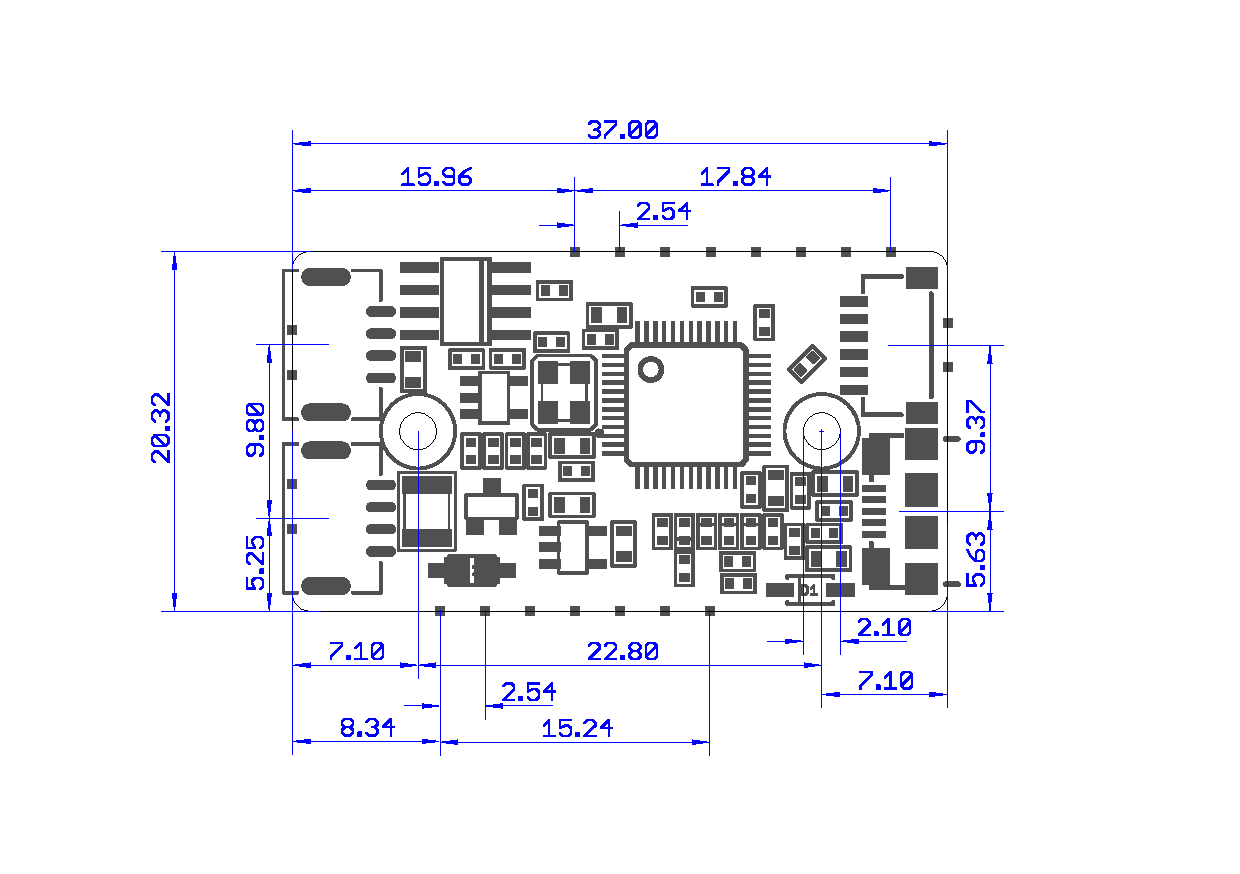
\includegraphics[width=1.2\textwidth]{babel_dimensions}}
	\caption{Physical dimensions of Babel.\label{fig:drawing}}
\end{figure}

\begin{figure}[hbtp]
	\centerline{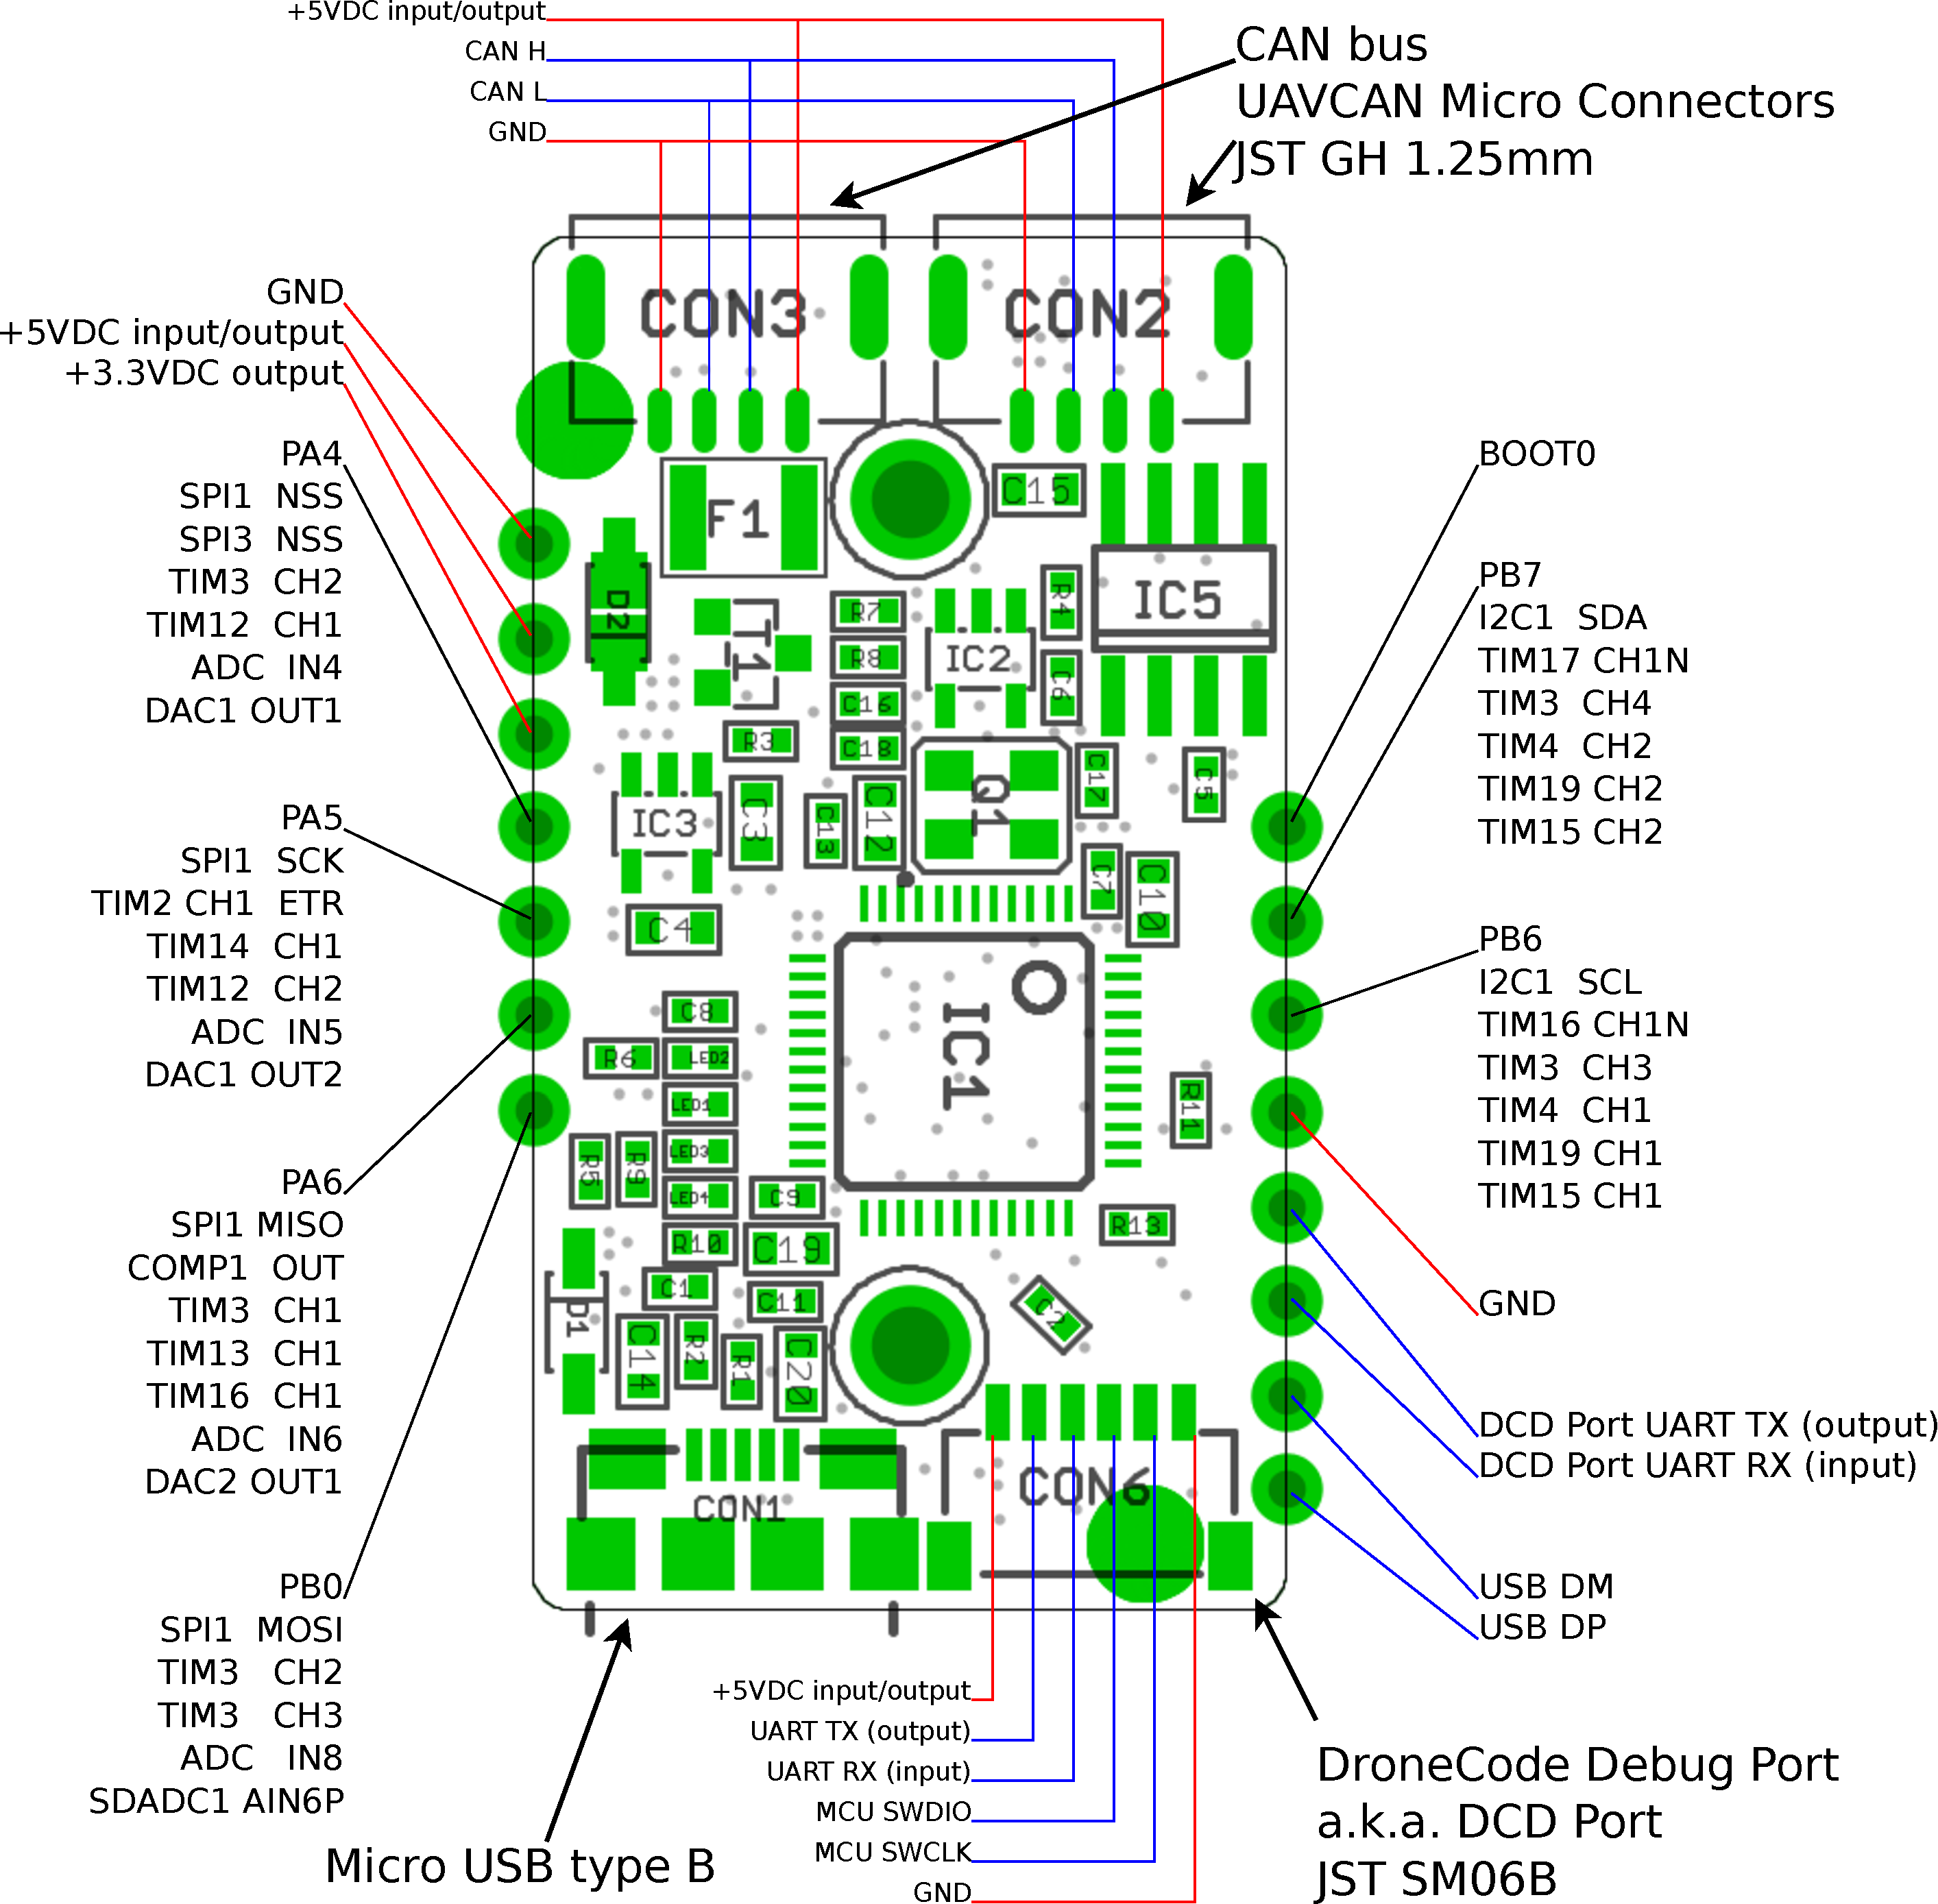
\includegraphics[width=1\textwidth]{pinout_annotated}}
	\vspace{2em}
	\caption{Babel pinout.\label{fig:pinout}}
\end{figure}

\chapter{Operating principles}

\section{Overview}

Babel keeps its CAN controller disabled by default in order to ensure that no unnecessary
interference with the CAN bus is introduced.
The CAN controller can be enabled, which is referred to as \emph{opening the channel}.
In this context, ``channel'' refers to the data tunnel between the CAN bus and a high-side
interface (either USB or UART).

When opening the channel, it is possible to explicitly specify the desired bit rate of the CAN bus.
If the CAN bit rate was not specified explicitly, Babel will use the value stored in the parameter
\CfgRef{can.bitrate}.
If the bit rate was specified explicitly, the parameter value will be automatically updated.

When the channel is opened, all of the buffers become flushed (i.e. cleared)
and the interface statistic counters get reset.
An attempt to open the channel when it is already opened is interpreted as if there was an implicit
close command before the channel is re-opened again.

Babel runs a single instance of an SLCAN protocol handler that can be attached either to the
USB CDC ACM interface (virtual serial port) or the physical UART interface.
By default, the UART interface is used.
If Babel detects that the USB interface is connected to a USB host,
it disconnects the SLCAN protocol handler from the UART port and attaches it to the USB CDC ACM port.
The reverse happens when the USB port becomes disconnected.
It is therefore impossible to use both USB and UART interfaces at the same time concurrently.

\section{Start up and initialization}

Immediately after powering on, the device starts the embedded bootloader (described in detail in the section
\ref{sec:bootloader}).
The bootloader awaits for external commands for a few seconds.
If no commands requesting it to download a new firmware image or wait longer were received,
and if a valid application (i.e. firmware) was found in the ROM,
the bootloader starts the application.
If no valid application is found in the ROM, the bootloader will wait for commands forever.

\section{LED indicators}

\newcommand{\LEDX}{{\rule{0.4em}{0.8em}}}
\newcommand{\LEDO}{{\rule{0.4em}{0.1em}}}

\newcommand{\ShowColor}[1]{{\color{#1}\rule{2em}{0.8em}}}

Babel is equipped with four separate LED indicators that reflect the current state of the device.
Their functions are summarized in the table \ref{table:led_indicators}.

\begin{ZubaxSimpleTable}{LED indicators}{|l l X|}\label{table:led_indicators}
    Color                     & Name               & Behavior \\
    \ShowColor{red} Red       & CAN power LED      & Glows when the CAN bus power output is enabled. \\
    \ShowColor{orange} Orange & CAN terminator LED & Glows when the CAN bus termination resistor is enabled. \\
    \ShowColor{blue} Blue     & Status LED         & See table \ref{table:status_led_behavior}. \\
    \ShowColor{green} Green   & CAN traffic LED    & Blinks once if at least one CAN frame was successfully
                                                     transmitted or successfully received in the last
                                                     25~milliseconds. Glows steadily when the intensity of CAN
                                                     traffic is higher than 40 frames per second.
                                                     The function of this LED is different while the bootloader
                                                     is running; see the section \ref{sec:bootloader}. \\
\end{ZubaxSimpleTable}

The behavior of the status LED is more complex than that of other indicators.
It is specified in the table \ref{table:status_led_behavior}.
Observe that there is one special mode that is used while the embedded bootloader is running.
The bootloader is documented separately in the section \ref{sec:bootloader}.

\begin{ZubaxSimpleTable}{Status LED behavior}{|l l X|}\label{table:status_led_behavior}
    Status & LED pattern (step 50 ms) & LED behavior \\

    Bootloader is running
    & \LEDX\LEDX\LEDX\LEDX\LEDX\LEDX\LEDX\LEDX\LEDX\LEDX\LEDX\LEDX\LEDX\LEDX\LEDX\LEDX\LEDX\LEDX\LEDX\LEDX
    & Glowing continuously.
      In this mode, the CAN traffic LED behaves as described in the section \ref{sec:bootloader}. \\

    CAN channel closed
    & \LEDO\LEDO\LEDO\LEDO\LEDO\LEDO\LEDO\LEDO\LEDO\LEDO\LEDO\LEDO\LEDO\LEDO\LEDO\LEDO\LEDO\LEDO\LEDO\LEDO
    & Turned OFF \\

    CAN channel open, normal operation
    & \LEDX\LEDO\LEDO\LEDO\LEDO\LEDO\LEDO\LEDO\LEDO\LEDO\LEDO\LEDO\LEDO\LEDO\LEDO\LEDO\LEDO\LEDO\LEDO\LEDO
    & Blinking 1 Hz \\

    CAN channel open, error passive
    & \LEDX\LEDO\LEDO\LEDO\LEDO\LEDX\LEDO\LEDO\LEDO\LEDO\LEDX\LEDO\LEDO\LEDO\LEDO\LEDX\LEDO\LEDO\LEDO\LEDO
    & Blinking 4 Hz \\

    CAN channel open, bus off
    & \LEDX\LEDO\LEDX\LEDO\LEDX\LEDO\LEDX\LEDO\LEDX\LEDO\LEDX\LEDO\LEDX\LEDO\LEDX\LEDO\LEDX\LEDO\LEDX\LEDO
    & Blinking 10 Hz \\
\end{ZubaxSimpleTable}

\chapter{SLCAN protocol}\label{sec:slcan}

SLCAN (also known as LAWICEL) is a quasi-standard protocol designed for tunneling CAN data (frames, commands and adapter status information) via serial links (UART or USB CDC ACM). Zubax Babel implements all mandatory SLCAN commands, so that its compatibility with third party software products that rely on SLCAN is ensured. A brief recap of standard SLCAN commands, prepared by Oliver Hartkopp, can be found in this document: \href{https://docs.zubax.com/zubax_babel/Generic_SLCAN_API.pdf}{Generic\_SLCAN\_API.pdf}.

SLCAN is an ASCII protocol, where the data is exchanged in blocks, each block may contain only printable ASCII characters and is terminated with either ACK (\fbox{$\backslash$r}, ASCII code 13) or NACK (\fbox{$\backslash$a}, ASCII code 7). Every block begins with a well-defined character which indicates what information the block is carrying; in this description we’re going to refer to this character as Block ID. Three types of blocks are defined:

\begin{itemize}
\item Command - these blocks are sent from the host to the adapter.
\item Response - these blocks are sent from the adapter to the host as a reaction to the corresponding command. Any command always results in exactly one response.
\item Notification - these blocks are generated by the adapter itself asynchronously.
\end{itemize}

All commands and notifications are always terminated with ACK (\fbox{$\backslash$r}). A response will be terminated with ACK if the command was executed successfully, and with NACK if the command failed or if the command ID could not be mapped to any known command handler.

Zubax Babel also implements an extension on top of SLCAN that allows the host to execute arbitrary CLI commands, sharing the same serial port with SLCAN. This feature is documented later in this section.

Note that some commands alter the configuration parameters of the adapter. All parameters can be stored into the non-volatile memory on the adapter, in which case they will be re-initialized to the saved values autimatically every time the adapter is turned on. The non-volatile memory feature is explained later in this section.

Keep in mind that Zubax Babel can be communicated with either via USB or via the DCD Port (UART), but not both at the same time. When USB is connected, only USB is used, the UART port is ignored. In order to use UART, USB must be disconnected.

Decent implementation of a host-side SLCAN driver in Python can be found in the \href{http://uavcan.org/Implementations/Pyuavcan/}{PyUAVCAN library}.
\clearpage

\section{SLCAN commands}

\subsection{CAN controller configuration}

\begin{ZubaxSimpleTable}{CAN controller configuration}{| l |  l | X |}
Block ID & Arguments & Purpose \\
\fbox{S} & 	Decimal number, see below & Set CAN bitrate. \\
\fbox{O} & None & Open CAN channel at the specified earlier bitrate in normal mode; re-open if already open. \\
\fbox{L} & None & Open CAN channel at the specified earlier bitrate in silent mode (listen only); re-open if already open. \\
\fbox{l} & None & Open CAN channel at the specified earlier bitrate in normal mode with loopback enabled; re-open if already open. \\
\fbox{C} & None & Close CAN channel; do nothing if channel is not open. \\
\fbox{M} & Any, not checked & This command is not applicable for Zubax Babel, it is implemented only for compatibility reasons. \\
\fbox{m} & Any, not checked & See \fbox{M}
\end{ZubaxSimpleTable}

All commands return \fbox{$\backslash$r} on success and \fbox{$\backslash$a} on failure. Commands that are implemented for compatibility always report success.

The command \fbox{S} accepts a non-negative decimal number which represents the desired CAN bitrate. If the channel is open, changes in bitrate will not take effect until it is re-opened again. The values are interpreted as follows:

\begin{ZubaxSimpleTable}{CAN bitrate}{| l |  X |}
Value & Interpretation, bits per second \\ 
0 & 10000 \\
1 & 20000 \\
2 & 50000 \\
3 & 100000 \\
4 & 125000 \\
5 & 250000 \\
6 & 500000 \\
7 & 800000 \\
8 & 1000000 \\
Any other & The number is interpreted as-is, no additional conversion is performed.\\
\end{ZubaxSimpleTable}

When the channel is open with loopback enabled, all transmitted frames will be sent back to the host, with the loopback flag set (if SLCAN flags are enabled). See more on this in the section dedicated to SLCAN notifications.

\subsection{CAN frame transmission}

In the command table, arguments are indicated as defined in the table below. Valid hexadecimal characters are the following:  \fbox{0123456789} \fbox{abcdef} \fbox{ABCDEF}.

\begin{ZubaxSimpleTable}{SLCAN arguments meaning}{| l |  X |}
Symbol & Meaning\\
\fbox{i} & 	Hexadecimal digit of a CAN ID \\
\fbox{d} & Hexadecimal DLC(Data Length Code) value \\ 
\fbox{*} & Useful data, encoded as a hexadecimal string, e.g. \fbox{0110FF} for the following sequence: 1, 16, 255. \\
\end{ZubaxSimpleTable}

\begin{ZubaxSimpleTable}{SLCAN command format}{| l |  l | l | X |}
Block ID & Arguments & Purpose & Example \\
\fbox{T} & \fbox{iiiiiiiid*} & Transmit 29-bit data frame & \fbox{T0123456780102030405060708$\backslash$r}\\
\fbox{t} & \fbox{iiid*} & Transmit 11-bit data frame & \fbox{t7FF0$\backslash$r}\\
\fbox{R} & \fbox{iiiiiiiid} & Transmit 29-bit RTR frame & \fbox{R1234f00d8$\backslash$r}(RTR frames have no payload)\\
\fbox{r} & \fbox{iiid} & Transmit 11-bit RTR frame & \fbox{r008$\backslash$r}(RTR frames have no payload)\\
\end{ZubaxSimpleTable}

All above listed commands may generate the following responses:

\begin{ZubaxSimpleTable}{Possible responses}{| l |  X |}
Response & Meaning \\
\fbox{Z$\backslash$r} & The frame has been successfully scheduled for transmission (for 29-bit ID) \\
\fbox{z$\backslash$r} & The frame has been successfully scheduled for transmission (for 11-bit ID) \\
\fbox{$\backslash$a} & The adapter could not transmit the frame (e.g. malformed frame, CAN channel is not open, etc.)\\
\end{ZubaxSimpleTable}

\subsection{Miscellaneous commands}

\begin{ZubaxSimpleTable}{Miscellaneous commands}{| l |  l | X |}
Block ID & Arguments & Purpose \\
\fbox{U} & Decimal number, see below & Set UART baud rate \\ 
\fbox{Z} & \fbox{0} or \fbox{1} & Enable (if 1) or disable (if 0) RX and loopback timestamping \\
\fbox{F} & None & Get and clear status flags \\ 
\fbox{V} & None & Get hardware and software version \\
\fbox{N} & None & Get unique ID (conventional SLCAN adapters return the serial number, which Zubax products may not have) \\
\end{ZubaxSimpleTable}
\clearpage

The command \fbox{U} accepts a non-negative decimal number which represents the desired UART baud rate. Changes will take effect shortly after the command was executed (typically within 100 milliseconds), no reboot is necessary; therefore, the host should adjust the baud rate of the serial port immediately after execution of this command. The number is interpreted as follows:

\begin{ZubaxSimpleTable}{Baudrate codes}{| l |  X |}
Value & Interpretation, baud per second \\
0 & 230400 \\ 
1 & 115200 \\
2 & 57600 \\
3 & 38400 \\
4 & 19200 \\
5 & 9600 \\
6 & 2400 \\
Any other & The number is interpreted as-is, no additional conversion is performed.
\end{ZubaxSimpleTable}

The following baud rates are supported: 2400, 9600, 19200, 38400, 57600, 115200 (this is the default), 230400, 460800, 921600, 1000000, 3000000. Other baud rates may also work too.

The command \fbox{Z} can be used to enable and disable timestamping. Changes will take effect shortly after the command was executed (typically within 100 milliseconds), no reboot is necessary. More on timestamping is in the following sections.

The command \fbox{F} produces \fbox{F??$\backslash$r}, where \fbox{??} is a hexadecimal bitmask, where the bits are assigned the following meanings:

\begin{ZubaxSimpleTable}{Command F bitmask meaning}{| l |  l | l | X |}
Bit & $2^{Bit}$ & Name & Meaning \\
3 & 8 & RX Overrun & The RX queue has overflowed at least once since the last invocation of the F command or since the channel was open. \\
5 & 32 & Error Passive & The CAN error counters have exceeded the error passive limit (refer to the CAN bus specification for details). \\
7 & 128 & Bus Off & The CAN controller is in the bus off mode (refer to the CAN bus specification for details).\\
\end{ZubaxSimpleTable}

Other bits should be ignored. Note that the CAN interface recovers from bus-off and other error states automatically.

The command \fbox{V} produces \fbox{V????$\backslash$r}, where the fields are hexadecimal numbers with the following meanings, in that order:

\begin{itemize}
\item Hardware version, major.
\item Hardware version, minor.
\item Software version, major.
\item Software version, minor.
\end{itemize}
 
 \clearpage
 
\section{SLCAN notifications}

Zubax Babel may generate SLCAN notifications only in the following cases:
\begin{itemize}
\item A CAN frame is received.
\item If loopback is enabled: a CAN frame has been successfully transmitted.
\end{itemize}

The format of notifications is the same as for CAN transmission commands:

\begin{ZubaxSimpleTable}{SLCAN notifications format}{| l | l | X |}
Block ID & Arguments & Purpose \\
\fbox{T} & \fbox{iiiiiiiid*} & Received or successfully transmitted a 29-bit data frame \\
\fbox{t} & \fbox{iiid*} & Same, 11-bit data frame \\
\fbox{R} & \fbox{iiiiiiiid} & Same, 29-bit RTR frame \\
\fbox{r} & \fbox{iiid} & Same, 11-bit RTR frame \\
\end{ZubaxSimpleTable}

Additionally, frame notification blocks may be extended with timestamp information and/or with flags, depending on the configuration.

When timestamping is enabled, frame notification blocks will be extended with four more hexadecimal characters, containing the time, in milliseconds, when they were received. The millisecond timestamp overflows every 60000 milliseconds (once a minute), so the valid values lie in the range from 0 to 59999, inclusive. The frame timestamp can be converted into the target clock domain, e.g. monotonic clock of the host system, using the \href{https://april.eecs.umich.edu/pdfs/olson2010.pdf}{Olson algorithm} (timestamp synchronization in PyUAVCAN is based on the Olson algorithm too). In loopback mode with timestamping enabled, the loopback frames will have the timestamp of the moment when they were delivered to the bus.

When SLCAN flags are enabled, frame notifications will be amended as follows:\
\begin{itemize}
\item Loopback frames will be appended the character \fbox{L} at the end of the block. This option allows the host to distinguish between received frames and the frames that were received from the bus.
\end{itemize}

For example, a frame \fbox{T12345678401234568} will be returned back as follows, depending on the configuration:

\begin{ZubaxSimpleTable}{SLCAN notification example}{| l |  l | X |}
Flags enabled & Timestamping enabled	& Representation \\
No & No & \fbox{T12345678401234568$\backslash$r} (no changes) \\
No & Yes & \fbox{T123456784012345680BED$\backslash$r} (transmission timestamp 3053 milliseconds) \\
Yes & No & \fbox{T12345678401234568L$\backslash$r} (added flag \fbox{L})\\
Yes & Yes & \fbox{T123456784012345680BEDL$\backslash$r} (both of the above) \\
\end{ZubaxSimpleTable}
\clearpage

\section{CLI extensions}

Zubax Babel implements an extension of the SLCAN protocol that allows it to run a conventional CLI shell over the same serial port that is used for SLCAN communications, while maintaining full compatibility with SLCAN.

A CLI command is a sequence of printable ASCII characters terminated with \fbox{$\backslash$r$\backslash$n} (ASCII codes 13, 10); the sequence must not be also a valid SLCAN command. Every CLI command returns a response that begins with the exact copy of the received command, terminated with \fbox{$\backslash$r$\backslash$n}, then followed by an arbitrary number of lines, each terminated with \fbox{$\backslash$r$\backslash$n}, and finalized with the ASCII END-OF-TEXT character (code 3) immediately followed by the final \fbox{$\backslash$r$\backslash$n}.

For example, a command \fbox{cfg   list} (the excessive spaces were added for demonstrational purposes) may produce the following response (non-printable characters are shown with escape sequences, e.g. \fbox{$\backslash$r}):

\begin{minted}[linenos = false]{yaml}
cfg   list  \r\n
can.bitrate           = 1000000     [10000, 1000000] (1000000)\r\n
can.power_on          = 0           [0, 1] (1)\r\n
can.terminator_on     = 0           [0, 1] (1)\r\n
slcan.timestamping_on = 1           [0, 1] (1)\r\n
slcan.flags_on        = 0           [0, 1] (0)\r\n
uart.baudrate         = 115200      [2400, 3000000] (115200)\r\n
\x03\r\n
\end{minted}

Where \fbox{$\backslash$x03} is the ASCII END-OF-TEXT character.

The facts that CLI commands and their responses are terminated with \fbox{$\backslash$r$\backslash$n} rather than plain \fbox{$\backslash$r}, and that a valid SLCAN command cannot be also a valid CLI command, can be used to distinguish SLCAN data from CLI data in real time. A compliant SLCAN driver that is capable of dealing with CLI extensions with virtually zero performance penalty can be found in the \href{http://uavcan.org/Implementations/Pyuavcan/}{PyUAVCAN library}.

CLI commands can be executed manually if the SLCAN port is open in a terminal emulator program (it is recommended to enable local echo, since SLCAN does not provide remote echo). Read this article for more info: \href{https://docs.zubax.com/usb}{USB command line interface}.
\clearpage

\subsection{CLI commands}

This section documents what CLI commands are implemented and how to use them.

\fbox{cfg}

This command allows to manage the configuration parameters. Execute without arguments to see usage info. More detailed description of configuration parameters is provided in a dedicated section. The following use cases are the most important:

\begin{itemize}
\item \fbox{cfg list} - list all configuration parameters, one per line, each line is formatted as follows:\\ \fbox{name = value [min, max] (default)}. Floating point parameters are rendered with explicit decimal separator, e.g.  \fbox{1.0} rather than \fbox{1}.
\item \fbox{cfg set <name> <value>} - assign the parameter a new value. The response may contain \fbox{Error:} followed by the description of the error in case of failure. It is recommended to execute \fbox{cfg list} afterwards to check if the value was updated.
\item \fbox{cfg save} - save the current configuration into the non-volatile memory. With firmware v1.1 this command became redundant and it should no longer be invoked manually,  because configuration parameters are saved into the non-volatile memory automatically upon modification.
\item \fbox{cfg erase} - remove the stored configuration from the non-volatile memory. Next restart will reset all parameters to defaults.
\end{itemize}

\fbox{zubax\textunderscore id}

When executed without arguments, returns the device identification information formatted as a YAML dictionary, such as name, version, unique ID, and so on. Example output:

\begin{minted}[linenos = false]{yaml}
product_id   : 'com.zubax.babel'
product_name : 'Zubax Babel'
sw_version   : '1.0'
sw_vcs_commit: 48923790
sw_build_date: Jun 20 2016
hw_version   : '1.0'
hw_unique_id : 'OAAyAA1XMkEzNjkgAAAAAA=='
hw_info_url  : http://device.zubax.com/device_info?uid=380032000D5732413336392000000000
hw_signature : 'SknsmA7XugU9pF/+NNOoU26Gdq9VvhO3O1Cw2qim17RXsU8yOISoKOdMIh4QIHtXr36sMfx
H397RlSNc0TtWDPOyA713z0k+v+ZY5PGXkRFiUfspnU/EJ8+r0url2dYp7NApx4lOklOgNgHrGCA6lPxA8UqoW
9jdqaASuqpFZKg='
\end{minted}

This command may also accept one argument, which must be the Base64 encoded RSA-1024 Certificate of Authenticity of the device. This use case does not serve any useful purpose during normal use of the device.
\clearpage

\fbox{stat}

Returns a YAML dictionary containing the immediate state information of the adapter. Example output:

\begin{minted}[linenos = false]{yaml}
open                  : true
state                 : error_active
receive_error_counter : 0
transmit_error_counter: 0
errors                : 0
bus_off_events        : 0
sw_rx_queue_overruns  : 0
hw_rx_queue_overruns  : 0
frames_tx             : 0
frames_rx             : 0
tx_queue_capacity     : 100
tx_queue_peak_usage   : 0
rx_queue_capacity     : 255
rx_queue_peak_usage   : 0
tx_mailbox_peak_usage : 0
bus_voltage           : 4.8
\end{minted}

The statistics is reset every time the channel is open. Note that it is kept intact after the channel is closed.

\fbox{bootloader}

Reboots the device into the bootloader, where it will wait forever for commands. What the bootloader is needed for and how to use it is documented in the dedicated section below.

\fbox{reboot}

Reboots the device.

\chapter{OEM applications}\label{sec:oem_applications}

Besides the primary role as a USB/UART-CAN adapter tool, Zubax Babel can be effectively applied as an integral part of a larger system or device, either as a CAN adapter or, if loaded with a user-developed firmware, in a completely different role. These use cases are referred to as OEM applications.

Additionally, Zubax Babel can be used as a prototyping platform for quick development of CAN (especially UAVCAN) dependent applications.

\section{SMD pads}

It is expected that OEM applications may require the adapter to be installed onto the custom PCB. For this reason, Zubax Babel is given SMD pads spaced at the standard 2.54 mm pitch. Soldering 0.1" pin connectors to the SMD pads will also enable easy integration with standard breadboards, as shown on the picture on the right.

The signals that are routed to the pads are shown on the diagram in the beginning of this document.

\section{Custom applications}

Please refer to the dedicated tutorial for detailed information about development of custom applications.

Zubax Babel is based on the microcontroller STM32F373CBT6; its main characteristics are outlined below:

\begin{itemize}
\item Core: ARM Cortex-M4F (with hardware floating point unit) at 72 MHz.
\item Flash memory capacity: 128 KB.
\begin{itemize}
\item First 32 KB are occupied by the bootloader and some auxiliary persistent data.
\item Following 94 KB are available for the user application.
\item Last 2 KB are reserved for non-volatile configuration storage.
\end{itemize}
\item RAM capacity: 24 KB.
\begin{itemize}
\item First 256 bytes are reserved for the bootloader operation.
\item Remaining 24320 bytes are available for the user application.
\end{itemize}
\end{itemize}

Custom applications can be loaded either directly via SWD, in which case great care should be taken to not accidentally erase the bootloader; or via the bootloader itself. More information about the bootloader can be gathered in the dedicated section.

\chapter{Configuration parameters}

Configuration parameters are stored in the non-volatile memory on the adapter. Stored parameters will be re-initialized to the saved values automatically every time the adapter is turned on. Changes in adapter configuration take effect shortly after the corresponding command changing them is executed, typically within 100 milliseconds, unless stated otherwise elsewhere. Some configuration parameters are aliased via dedicated standard SLCAN commands.

Starting from firmware version v1.1, configuration parameters are stored into the non-volatile memory automatically after modification.

% name, SLCAN alias, takes effect at, min, max, default, note
\newcommand\CfgParamIndexEntry[7]{%
    \CfgDef{#1} & \footnotesize{#2} & \footnotesize{#3} & \footnotesize{\CfgListReferences{#1}} &
    \footnotesize{#4} & \footnotesize{#5} & \footnotesize{#6} & \footnotesize{#7}
    \tabularnewline
}%
\newenvironment{CfgParamIndex}[1]{%
    \begin{ZubaxTableWrapper}{#1}
    \setlength\tabcolsep{2.5pt}
    \begin{ZubaxWrappedTable}{@{} l c l l | c c c | X @{}}
    Name & \makecell[cb]{SLCAN\\alias} & \makecell[lb]{Takes\\effect at} & Pages & Min & Max & Def. & Description \\
}{%
    \end{ZubaxWrappedTable}
    \end{ZubaxTableWrapper}
}

\begin{CfgParamIndex}{Configuration parameter index}

\CfgParamIndexEntry{can.bitrate}{S}{channel open}{10\,000}{1\,000\,000}{1\,000\,000}
{CAN bus bit rate, in bit/s.}

\CfgParamIndexEntry{can.power+on}{}{immediately}{0}{1}{1}
{Enable CAN bus power output.}

\CfgParamIndexEntry{can.terminator+on}{}{immediately}{0}{1}{1}
{Enable the embedded CAN bus termination resistor.}

\CfgParamIndexEntry{slcan.timestamping+on}{Z}{immediately}{0}{1}{1}
{Time stamp all incoming and outgoing CAN frames.}

\CfgParamIndexEntry{slcan.flags+on}{}{immediately}{0}{1}{0}
{Enable flags for SLCAN notifications (SLCAN protocol extension).}

\CfgParamIndexEntry{uart.baudrate}{U}{immediately}{2400}{3\,000\,000}{115200}
{Baud rate of the UART port.}

\end{CfgParamIndex}

\chapter{Embedded bootloader}\label{sec:bootloader}

The embedded bootloader enables firmware update via the following protocols and interfaces:

\begin{ZubaxSimpleTable}{Bootloader protocols and interfaces}{| X[2] | X[2] | X[7] | X[5] |}
Interface & Parameters & Protocol & Note \\
USB & CDC ACM & YMODEM, XMODEM, XMODEM-1K (autodetect) & When connected, DCD Port is inactive \\
DCD port (UART) & 115200-8N1 (fixed) & Same as USB CDC ACM & 	Available only while USB is disconnected \\
\end{ZubaxSimpleTable}

\section{CLI commands}

\fbox{reboot}

Restarts the bootloader.

\fbox{zubax\textunderscore id}

Same as if it was executed in the application’s CLI, with the addition of at least the following fields:
\begin{itemize}
\item \fbox{bl\textunderscore version} - bootloader version, major and minor.
\item \fbox{bl\textunderscore vcs\textunderscore commit} - git commit hash of the bootloader sources.
\item \fbox{mode} -  set to the string \fbox{bootloader} to indicate that the bootloader is running.
\end{itemize}

\fbox{state}

Prints the bootloader state, which can be one of the following:

\begin{ZubaxSimpleTable}{Bootloader states}{| l |  l | X |}
State ID & State name & Comment \\
0 & \fbox{NoAppToBoot} & There is no valid application to boot; the bootloader will be waiting for commands forever. \\
1 & \fbox{BootDelay} & 	The bootloader will start the application in a few seconds, unless the boot is cancelled or a firmware update is requested. \\
2 & \fbox{BootCancelled} & There is a valid application to boot, however, boot was cancelled by an external command. \\
3 & \fbox{AppUpgradeInProgress} & Application is currently being upgraded. If interrupted, the bootloader will go into \fbox{NoAppToBoot}. \\
4 & \fbox{ReadyToBoot} & The application is already booting. This state is very transient and is left automatically as soon as possible. \\ 
\end{ZubaxSimpleTable}

\begin{figure}[H]
	\centerline{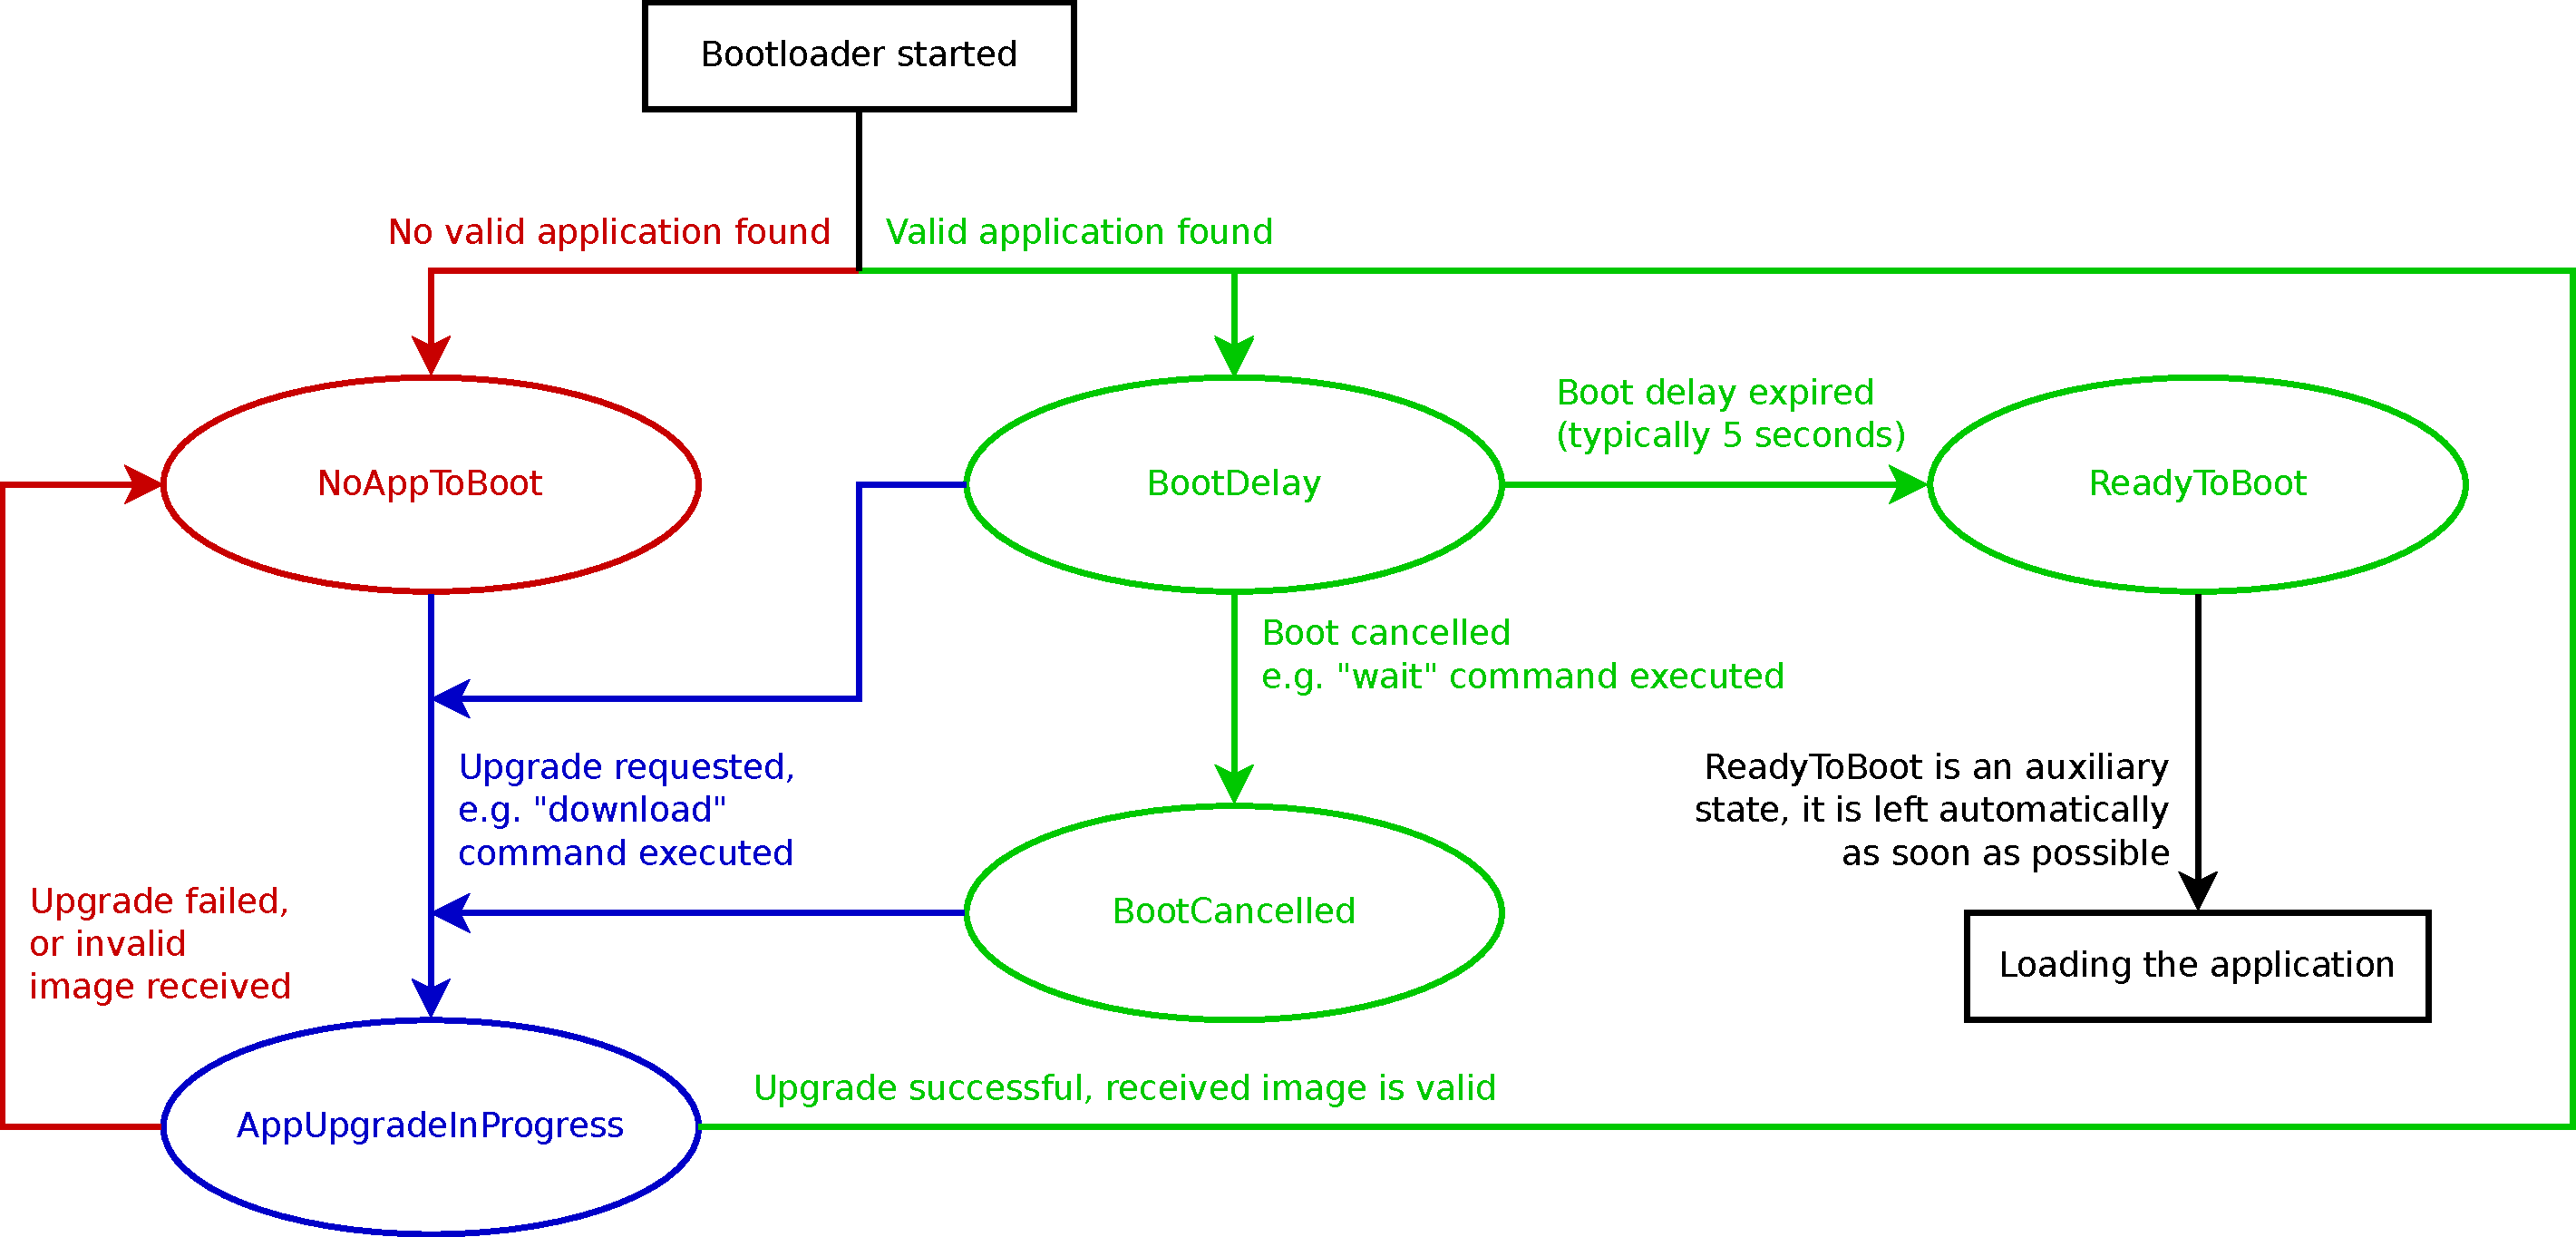
\includegraphics[width=1\textwidth]{bootloader_state_machine}}
	\caption{Bootloader state machine.\label{bootloader_state_machine}}
\end{figure}

\fbox{wait}

Do not boot the application.

\fbox{download}

Start the serial receiver and prepare to receive the new firmware image as a flat binary via the serial link using either YMODEM, XMODEM, or XMODEM-1K. There are heaps of software products and scripts that support these protocols. For instance, the standard program \fbox{sz} can be used as follows:

\begin{minted}[linenos = false]{yaml}
sz -vv --ymodem --1k $file > $port < $port
\end{minted}

If the application was successfully received and CRC verification confirmed that it is not damaged, the bootloader will automatically transition into the state \fbox{BootDelay}.

\iffalse

\chapter{Accessories}

Zubax Babel can be used with the following accesories:
\begin{itemize}
\item \href{https://github.com/Zubax/zubax_babel/tree/master/hardware/enclosure}{Enclosure (suitable for 3D printing)}
\item \href{https://docs.zubax.com/uavcan#UAVCAN_Micro_Patch_Cable}{UAVCAN Micro Patch Cable}
\item \href{https://docs.zubax.com/uavcan#UAVCAN_Micro_to_DF13_Adapter_Cable}{UAVCAN Micro to DF13 Adapter Cable}
\item \href{https://docs.zubax.com/zubax_babel#UAVCAN_Micro_to_D-SUB_DB9F_CAN_Adapter_Cable}{UAVCAN Micro to D-SUB DB9F CAN Adapter Cable}
\end{itemize}

The acessories can be purchased from \href{https://zubax.com/sales-network}{our distributors}.

\chapter{Links}

\begin{itemize}
\item \href{http://shop.titaneliteinc.com/index.php?route=product/product&product_id=1004}{Purchase}
\item \href{https://github.com/Zubax/zubax_babel}{Source repository (includes 3D printable enclosure models)}
\item \href{http://zubax.com/product/zubax-babel}{Product description}
\end{itemize}

\fi

\end{document}
